\documentclass[../SOP.tex]{standalone}

\usepackage{tikz}

\def\layersep{1.5cm}

\begin{document}
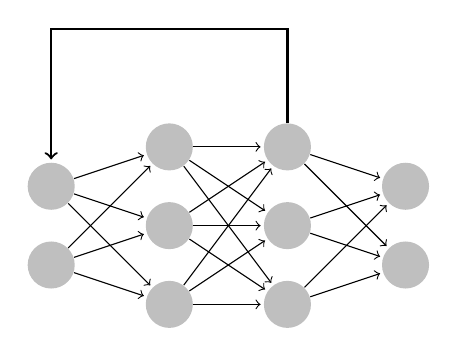
\begin{tikzpicture}[shorten >=1pt,->,draw=black,node distance=\layersep]
  \tikzstyle{every pin edge}=[<-, shorten <= 1pt]
  \tikzstyle{neuron}=[circle,fill=black!25,minimum size=17pt,inner sep=0pt]
  \tikzstyle{annot} = [text width=4em, text centered]


  \foreach \name / \y in {1,...,2}
    \node[neuron] (I-\name) at (0,-\y) {};

  \foreach \name / \y in {1,...,3}
    \path[yshift=0.5cm]
    node[neuron] (Ha-\name) at (\layersep,-\y) {};

  \foreach \name / \y in {1,...,3}
    \path[yshift=0.5cm]
    node[neuron] (Hb-\name) at (2*\layersep,-\y) {};

  \foreach \name / \y in {1,...,2}
    \node[neuron] (O-\name) at (3*\layersep,-\y) {};

  \foreach \source in {1,...,2}
    \foreach \dest in {1,...,3}
    \path (I-\source) edge (Ha-\dest);

  \foreach \source in {1,...,3}
    \foreach \dest in {1,...,3}
    \path (Ha-\source) edge (Hb-\dest);

  \foreach \source in {1,...,3}
    \foreach \dest in {1,...,2}
    \path (Hb-\source) edge (O-\dest);

    \draw[thick] (Hb-1) -- (2*\layersep, 1) -- (0,1) -- (I-1);
\end{tikzpicture}
\end{document}
